\documentclass[11pt,a4paper]{article}
\usepackage[a4paper,margin=2.5cm]{geometry}
\usepackage{microtype}
\usepackage{amsmath}
\usepackage{graphicx}
\usepackage{booktabs}
\usepackage{multirow}
\usepackage{xcolor}
\usepackage[font=small,labelfont=bf,skip=4pt]{caption}
\usepackage[round,authoryear]{natbib}
\usepackage{titlesec}
\usepackage{enumitem}
\usepackage{hyperref}
\usepackage{float}

\titlespacing*{\section}{0pt}{1.0ex plus .3ex}{0.5ex}
\titlespacing*{\subsection}{0pt}{0.8ex plus .2ex}{0.3ex}
\titleformat*{\section}{\large\bfseries}
\titleformat*{\subsection}{\normalsize\bfseries}
\setlength{\parskip}{0.25em}
\setlength{\parindent}{0pt}
\setlength{\textfloatsep}{8pt plus 2pt}
\setlength{\floatsep}{6pt plus 2pt}
\setlength{\intextsep}{6pt plus 2pt}
\newcommand{\pkg}[1]{\texttt{#1}}
\newcommand{\para}[1]{\textbf{#1}\ }

\begin{document}

% ------------------------------------------------------------------ title page
\begin{titlepage}
\centering
\vspace*{4cm}
{\LARGE\bfseries Clothing Classification on Fashion-MNIST\par}
\vspace{0.4cm}
{\large Decision trees, tree ensembles and a deep learning design\par}
\vspace{2.5cm}
{\large Thijs Niekerk \quad (SNR 2125613)\par}
\vspace{0.15cm}
{\large Pjotr Martens \quad (SNR 2080478)\par}
\vfill
{Machine Learning Analytics, Final Project\par}
\vspace{0.15cm}
{Tilburg School of Economics and Management, Tilburg University\par}
\vspace{0.15cm}
{October 2026\par}
\vspace*{1.5cm}
\end{titlepage}
\setcounter{page}{1}

% ------------------------------------------------------------------ 1
\section{Data and set-up}
\label{sec:data}
Fashion-MNIST \citep{xiao2017} has 70{,}000 grayscale $28\times28$ images of ten balanced clothing classes (60{,}000 for training, 10{,}000 for testing). We flatten each image into 784 pixel values and scale them to $[0,1]$. The average images of the classes (Figure~\ref{fig:data}) show that Pullover, Coat and Shirt have almost the same shape (their mean images correlate 0.95--0.97), with T-shirt closest to Shirt (0.87). Labelling a test image by its closest average image gives 67.7\% accuracy, but an F1 score of only 0.26 for Shirt. k-means with ten clusters (Figure~\ref{fig:kmeans}) puts at least 84\% of the Trouser, Sneaker and Ankle boot images in one cluster each, but 47\% of the T-shirt, Pullover, Coat and Shirt images land in a cluster dominated by one of the other three, so we expect these upper-body classes to be the hard part. Finally, neighbouring pixels are strongly related (horizontal neighbours correlate 0.78, pixels seven columns apart 0.32), and 105 border pixels are zero in over 90\% of the images. Trees are not affected by rescaling and rarely split on empty pixels, so we do no further preprocessing.

\begin{figure}[h]
\centering
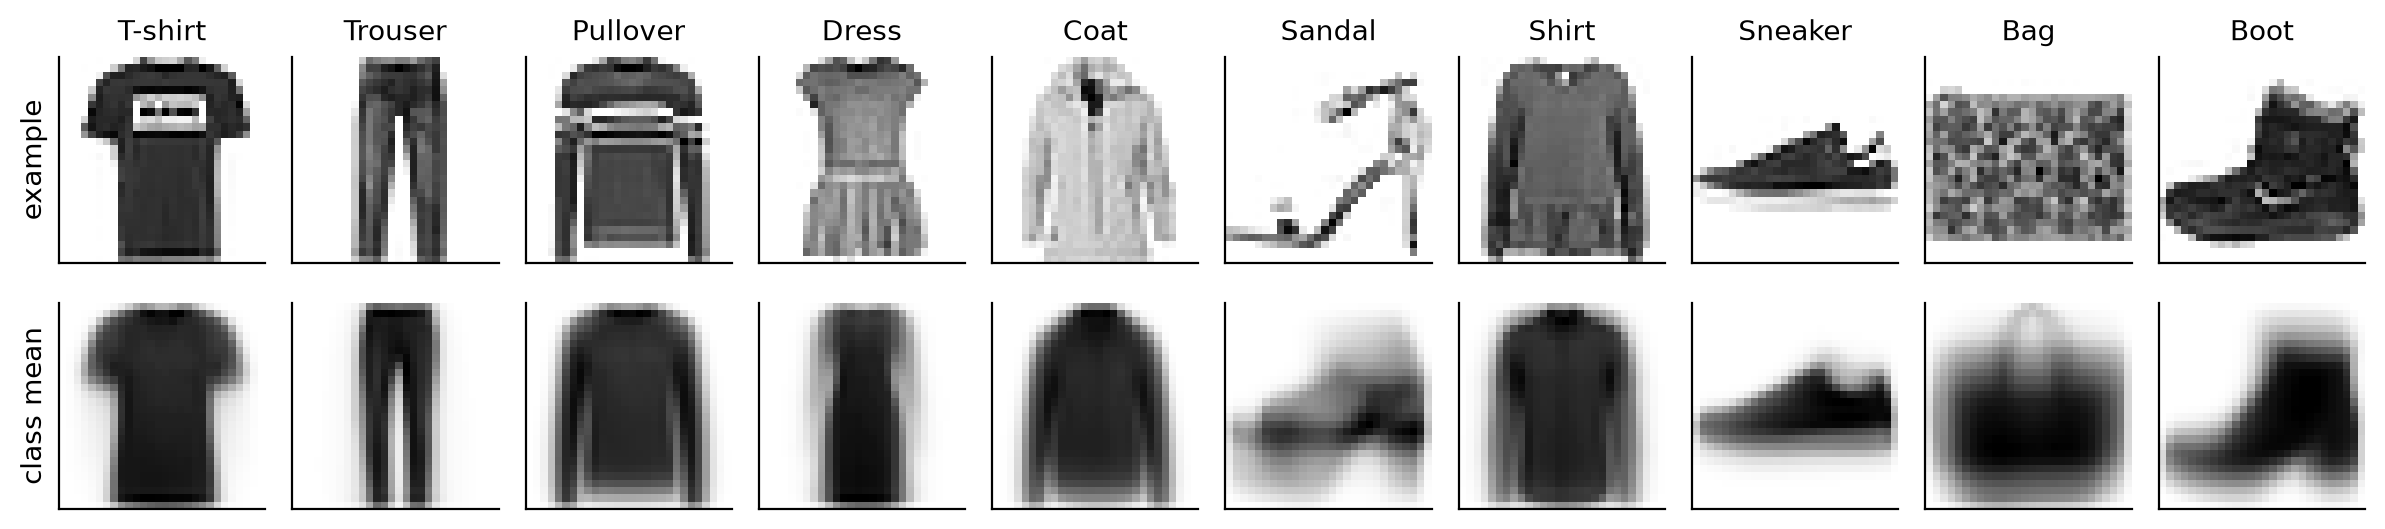
\includegraphics[width=0.74\linewidth]{figures/data_overview.png}
\caption{One training image (top) and the average training image (bottom) of every class.}
\label{fig:data}
\end{figure}

All hyperparameters are tuned with 3-fold cross-validation (CV) on the 60{,}000 training images. Final models are refitted on all training images and every model is evaluated once on the same untouched test set. Next to accuracy, which is fair with balanced classes, we report confusion matrices and for each class the F1 score $F_1=2PR/(P+R)$, which combines precision $P$ (the share of images given a label that truly belong to it) and recall $R$ (the share of a class that is recognised); the average F1 is the mean of the ten per-class scores.

% ------------------------------------------------------------------ 2
\section{Part 1: decision tree and tree ensemble}
\subsection{Decision tree (1a)}
\label{sec:tree}
We use \pkg{DecisionTreeClassifier} \citep{sklearn} with the Gini index and compare two stopping criteria (maximum depth, minimum images per leaf) as well as cost-complexity pruning. An unrestricted tree fits the training data perfectly but reaches only 78.9\% in CV (Figure~\ref{fig:tuning}a): it overfits. A depth of 12 with at least 10 images per leaf gives 81.2\%; pruning with $\alpha=2\cdot10^{-4}$ does slightly better (81.5\%), so we use the pruned tree (270 leaves), which reaches 80.8\% test accuracy (Table~\ref{tab:results}). Its first split asks whether one pixel near the top of the image is empty, which separates footwear (and some bags) from clothing.

The errors are very uneven (Figure~\ref{fig:cm}a, Table~\ref{tab:perclass}). Trouser, Bag, Sandal and Ankle boot reach F1 scores above 0.90, but Shirt (0.54), Coat (0.67) and Pullover (0.68) do not, and 56\% of all mistakes are confusions among the four upper-body classes. Only 499 of the 1{,}000 test shirts are recognised, as Section~\ref{sec:data} suggested. A tree only checks single pixels against a threshold, which works when one pixel is decisive (the gap between trouser legs) but not when classes differ in a collar or buttons that sit in a slightly different place in every image. The tree thus has two problems: \emph{high variance} (the gap between training and CV accuracy) and a \emph{bias} from looking at single raw pixels.

\subsection{Ensemble method (1b)}
\label{sec:ensemble}
\para{Choice and motivation.} Tree ensembles come in two kinds. Bagging trains many deep trees independently and averages them, which mainly reduces variance; boosting adds small trees one by one, each correcting the errors of the previous ones, which mainly reduces bias. Section~\ref{sec:tree} showed that our single decision tree mainly suffers from variance: grown fully it fits the training data perfectly (100\%) but reaches only 78.9\% in CV. Bagging is the natural remedy for this. Boosting mainly targets bias instead, has more settings that interact (learning rate, number of rounds, tree depth) and has to build its trees one after the other. As references we fit two boosting models with default settings: \pkg{GradientBoostingClassifier} and XGBoost.

Within bagging we choose a \textbf{random forest} \citep{breiman2001}. Averaging trees does not change the bias and never increases the variance, but how much it lowers the variance depends on how correlated the trees are. With 784 correlated pixels, plain bagged trees tend to use the same strong pixels near the root and become very similar. A random forest considers only a random subset of $m<p$ pixels at every split, so a strong pixel cannot dominate most trees and the trees become less correlated.

\para{Implementation.} We use \pkg{RandomForestClassifier} with fully grown trees. Its key setting is $m$ (\pkg{max\_features}), the number of pixels, drawn at random from all $p=784$, that each split can consider. We first tune the number of trees with $m=\sqrt{p}=28$: CV accuracy rises quickly up to 50 trees (87.7\%) and only slowly after that (88.1\% at 200 trees, against 87.8\% on the test set later, Figure~\ref{fig:tuning}b), and more trees cannot cause overfitting, so the final forest has 200 trees. Because 50 trees are already enough to compare settings, and much faster, we then vary $m$ from 7 to 112 with 50 trees each and compare with plain bagging ($m=p=784$, \pkg{BaggingClassifier}) of the same size (Figure~\ref{fig:tuning}c). CV accuracy rises steadily from 86.9\% at $m=7$ via 87.7\% at $m=28$ to 87.9\% at $m=112$, but drops to 87.1\% for plain bagging. The single trees show why: with $m=7$ they are weak (73.0\% accuracy) but their errors are less correlated (0.33), bagged trees are stronger (77.6\%) but more correlated (0.41), and $m=28$ lies in between (75.9\%, 0.36). Since $m=112$ beats $m=28$ by only 0.3 points, about the spread between folds, while training a 200-tree forest takes 4.1 times as long, we keep $m=\sqrt{p}=28$, the standard choice for classification and the default in \pkg{scikit-learn}.


\para{Expected versus observed effects.} We expected the forest to remove most of the variance but not the pixel-level bias, so the same classes should stay difficult, and this is what we found. Accuracy rises from 80.8\% to 87.8\%: the forest corrects 965 of the tree's mistakes and makes 263 new ones. Every class improves (Shirt F1 0.54$\to$0.65), but the share of errors among the upper-body classes grows from 56\% to 65\% (Figure~\ref{fig:cm}b): the forest mostly removed the scattered mistakes. To test robustness, for example to lower-quality photos, we add Gaussian noise ($\sigma=0.1$) to every test pixel: the tree drops to 45.9\%, since splits such as its first one test whether a pixel is empty, while the forest, which averages over many pixels, keeps 77.1\%. SHAP values of the final forest, computed with \pkg{TreeExplainer} on 1{,}000 test images (100 per class), and its impurity-based importance agree (correlation 0.91, Figure~\ref{fig:importance}): the forest relies on outline pixels at the neckline, the sleeves and the gap between trouser legs. On the first CV fold, a forest on only the 400 pixels with the highest SHAP values does as well as one on all 784 pixels (87.3\%), and 100 pixels still give 84.8\%. The pixels that push a shirt towards Shirt lie at the collar, along the button line and at the hem (Figure~\ref{fig:importance}c), small details that move from image to image. Gradient boosting with default settings (depth-3 trees) stays below the forest (86.7\%, 71.0\% with noise); its training and test accuracy were close and still rising after 100 rounds (Figure~\ref{fig:gb}), so its small trees are limited by bias. XGBoost \citep{xgboost} with default settings does beat the forest (89.8\%, 78.1\% with noise). Its deeper (depth-6) trees with penalised leaf values probably lower the bias while keeping the variance in check: it fits 99.97\% of the training images and still generalises better. So the forest beats boosting with small trees, confirming that variance was the tree's main problem, but part of the remaining error is bias that a well-built tree ensemble can still reduce.

\para{Difficulties.} \pkg{GradientBoostingClassifier} fits ten trees per round (one per class) on a single core and took 97 minutes, so we could not tune it; for a fair comparison XGBoost is not tuned either. SHAP values are slow for 200 deep trees, so we split the computation over all processor cores.

% ------------------------------------------------------------------ 3
\section{Part 2: a deep learning approach}
\subsection{Shortcomings of the tree-based approach (2c)}
(i) \textbf{No use of image structure.} Every split looks at one pixel, so the correlation between neighbours is ignored and a collar needs a long chain of splits. (ii) \textbf{No position invariance.} What is learned about one pixel does not carry over to its neighbour, so a collar two pixels further left must be learned again. (iii) \textbf{Remaining bias.} Beyond about 50 trees accuracy hardly improves, yet 65\% of the remaining mistakes are upper-body confusions ; XGBoost, which also reduces bias, does better (89.8\%) but still splits on single pixels and keeps Shirt as its weakest class by far (F1 0.71). The model needs better features, not more trees.

\subsection{Proposed design: a convolutional neural network (2d)}
These shortcomings lead us to a \textbf{convolutional neural network} (CNN) \citep{lecun1998}, which we would build in Keras (Table~\ref{tab:cnn} in Appendix~\ref{app:results}). Small $3\times3$ filters on the $28\times28$ image learn local patterns such as edges and collar shapes, using the strong correlation between neighbouring pixels that the trees ignore (i). Each filter slides over the whole image, so a pattern is found wherever it appears, and max pooling per $2\times2$ region makes the output less sensitive to small shifts (ii). The second convolution combines these patterns into larger parts such as sleeves and collars, the higher-level features the forest could not build (iii). Pooling twice, to $7\times7$, halves the dense layer compared with a single block. To avoid overfitting, we combine: dropout (randomly turns off neurons, acting like an ensemble of many smaller networks, similar to a random forest), an L2 penalty (Ridge), early stopping (stops training before the model starts memorizing instead of generalizing), and data augmentation (flipping images or shifting them a couple of pixels, so the model learns that the same object still looks the same when moved slightly, (ii)). A fully connected network or an autoencoder works on flattened pixels and keeps shortcomings (i) and (ii); a network on the pooled $14\times14$ image loses the small details that separate Shirt from Pullover.



\subsection{Implementation and expected results (2e)}
We reshape the images to $28\times28\times1$, one-hot encode the labels and use the Adam optimiser with cross-entropy loss. We train with batch size 32 for at most 30 epochs, hold out a stratified 10\% of the training images for validation and stop once the validation loss has not improved for three epochs, keeping the best weights. Dropout, L2 weight and filter counts are tuned on the validation set, using the training curves to spot overfitting. We test once with the measures of Table~\ref{tab:results} and compare with a fully connected network (784--150--60--10) trained the same way.

We expect about 92\% test accuracy: eight of the ten two-block CNNs in the public benchmark reach 91.6--93.9\% \citep{fmnistbenchmark}. Most of the gain should go to Shirt, Pullover and Coat, but Shirt will stay the weakest class, as some images are ambiguous even for people (83.5\% human accuracy, \citealp{fmnistbenchmark}). A single untuned run of this design (Appendix~\ref{app:cnn}) reaches 90.7\% (Shirt F1 0.74) against 86.6\% for a fully connected network; tuning, which we did not do, should close most of the gap to the benchmark.

\section{Conclusion}
A single decision tree reaches 80.8\% test accuracy. It overfits strongly and, checking single pixels, struggles to tell T-shirts, pullovers, coats and shirts apart. A random forest removes most of this variance: it makes 37\% fewer errors, is far more robust to noise and beats plain bagging and gradient boosting with small trees. XGBoost does better (89.8\%), so part of the remaining error is bias that deeper, penalised boosted trees can still reduce. Most remaining mistakes are confusions between upper-body garments, which come from working with single pixels. A CNN learns local features that tolerate small shifts; a single untuned run of our design already reaches 90.7\%, above every tree model, so we expect a tuned version to cut the remaining error clearly, although some shirts will stay ambiguous at this resolution.

% ------------------------------------------------------------------ references
\begin{thebibliography}{99}
\setlength{\itemsep}{1pt}
\small
\bibitem[Breiman(2001)]{breiman2001} Breiman, L. (2001). Random forests. \textit{Machine Learning}, 45(1), 5--32.
\bibitem[Chen and Guestrin(2016)]{xgboost} Chen, T. and Guestrin, C. (2016). XGBoost: a scalable tree boosting system. \textit{Proceedings of the 22nd ACM SIGKDD International Conference on Knowledge Discovery and Data Mining}, 785--794.
\bibitem[LeCun et~al.(1998)]{lecun1998} LeCun, Y., Bottou, L., Bengio, Y. and Haffner, P. (1998). Gradient-based learning applied to document recognition. \textit{Proceedings of the IEEE}, 86(11), 2278--2324.
\bibitem[Pedregosa et~al.(2011)]{sklearn} Pedregosa, F. et al. (2011). Scikit-learn: machine learning in Python. \textit{Journal of Machine Learning Research}, 12, 2825--2830.
\bibitem[Xiao et~al.(2017)]{xiao2017} Xiao, H., Rasul, K. and Vollgraf, R. (2017). Fashion-MNIST: a novel image dataset for benchmarking machine learning algorithms. \textit{arXiv:1708.07747}.
\bibitem[Zalando Research(2026)]{fmnistbenchmark} Zalando Research (2026). Fashion-MNIST repository, benchmark table. \url{https://github.com/zalandoresearch/fashion-mnist}, accessed October 2026.
\end{thebibliography}

% ------------------------------------------------------------------ appendix
\clearpage
\appendix
\section{Figures and tables}
\label{app:results}

\begin{table}[H]
\centering
\small
\begin{tabular}{lcccccc}
\toprule
 & Test & Average & Shirt & \multicolumn{2}{c}{With noise} & Training \\
\cmidrule(lr){5-6}
Model & acc. & F1 & F1 & $\sigma=0.1$ & $\sigma=0.2$ & time \\
\midrule
Closest average image (baseline) & 67.7\% & 0.672 & 0.26 & -- & -- & $<$1 s \\
Decision tree (pruned)           & 80.8\% & 0.807 & 0.54 & 45.9\% & 36.0\% & 44 s \\
Random forest (200 trees)        & 87.8\% & 0.877 & 0.65 & 77.1\% & 60.4\% & 54 s \\
Gradient boosting (default)      & 86.7\% & 0.866 & 0.64 & 71.0\% & 55.5\% & 97 min \\
XGBoost (default)                & 89.8\% & 0.898 & 0.71 & 78.1\% & 65.7\% & 4 min \\
\bottomrule
\end{tabular}
\caption{Test results. \emph{With noise}: Gaussian noise with standard deviation $\sigma$ added to the test images. Training on all training images on the same laptop with 8 cores (the forest and XGBoost use all of them, the other models one).}
\label{tab:results}
\end{table}

\begin{figure}[H]
\centering
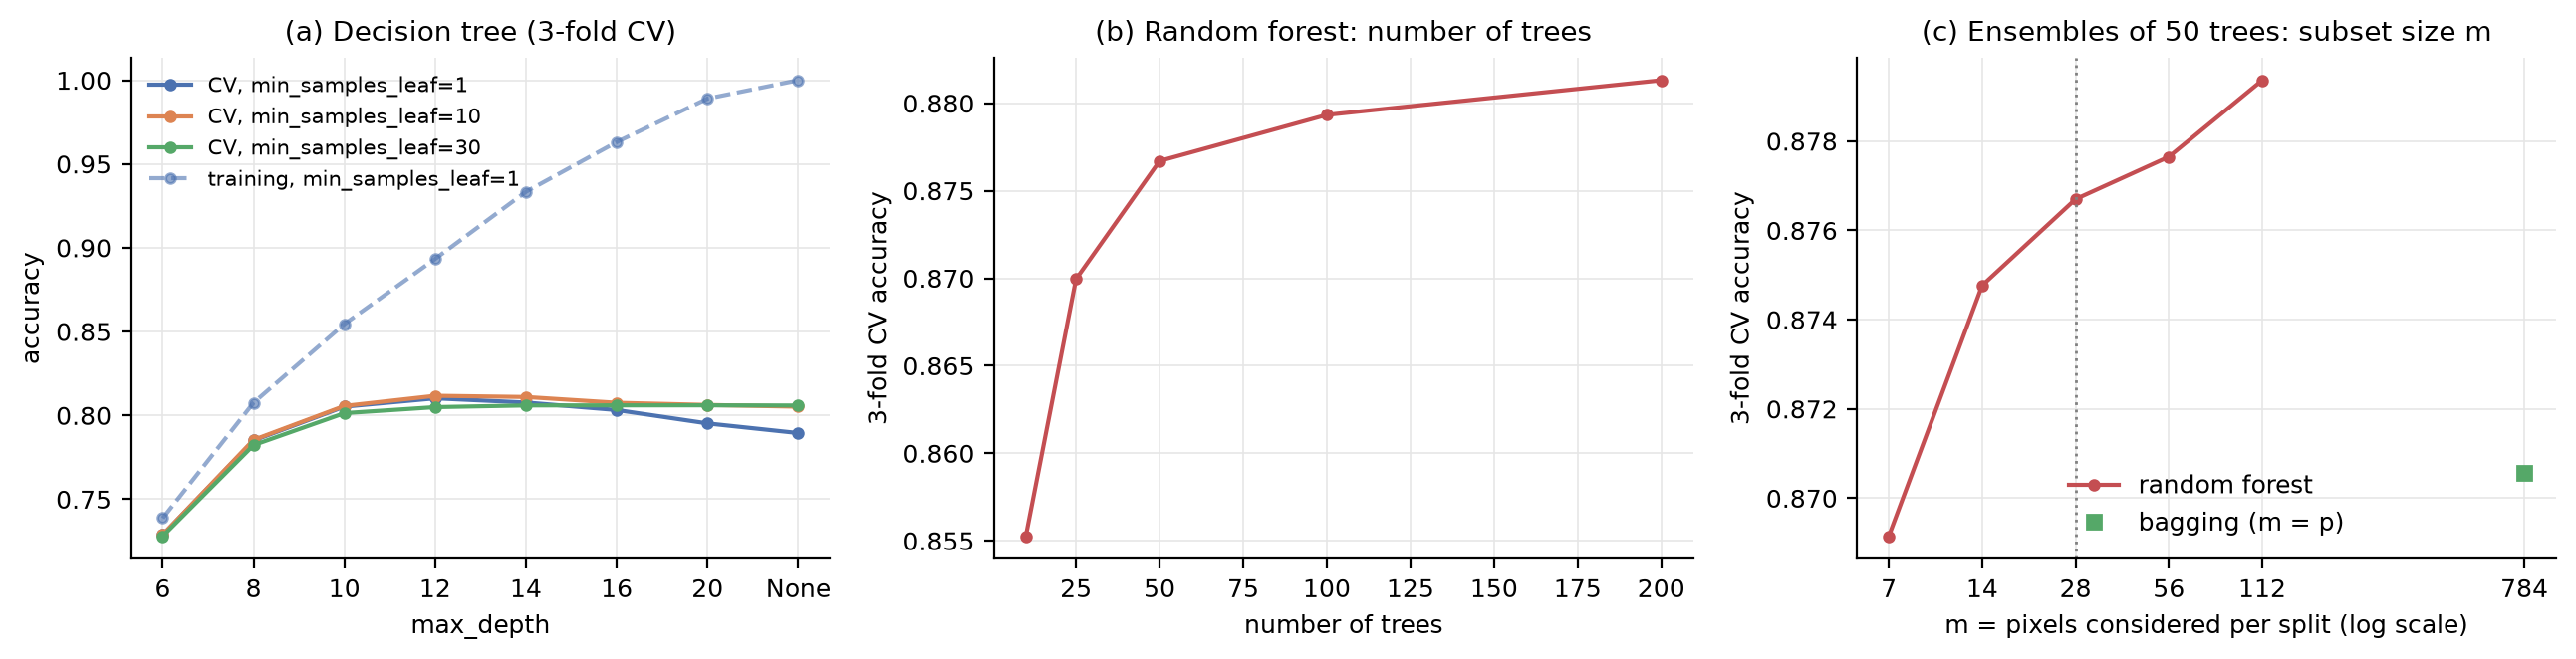
\includegraphics[width=\linewidth]{figures/tuning_curves.png}
\caption{Model selection. (a) Decision tree: 3-fold CV accuracy against \pkg{max\_depth} for three values of \pkg{min\_samples\_leaf}, and training accuracy for \pkg{min\_samples\_leaf}$=1$. (b) Random forest ($m=28$): 3-fold CV accuracy against the number of trees. (c) Ensembles of 50 trees: 3-fold CV accuracy against the number $m$ of pixels considered per split; the square is bagging ($m=p$), the dotted line the chosen $m=\sqrt{p}$.}
\label{fig:tuning}
\end{figure}

\begin{figure}[H]
\centering
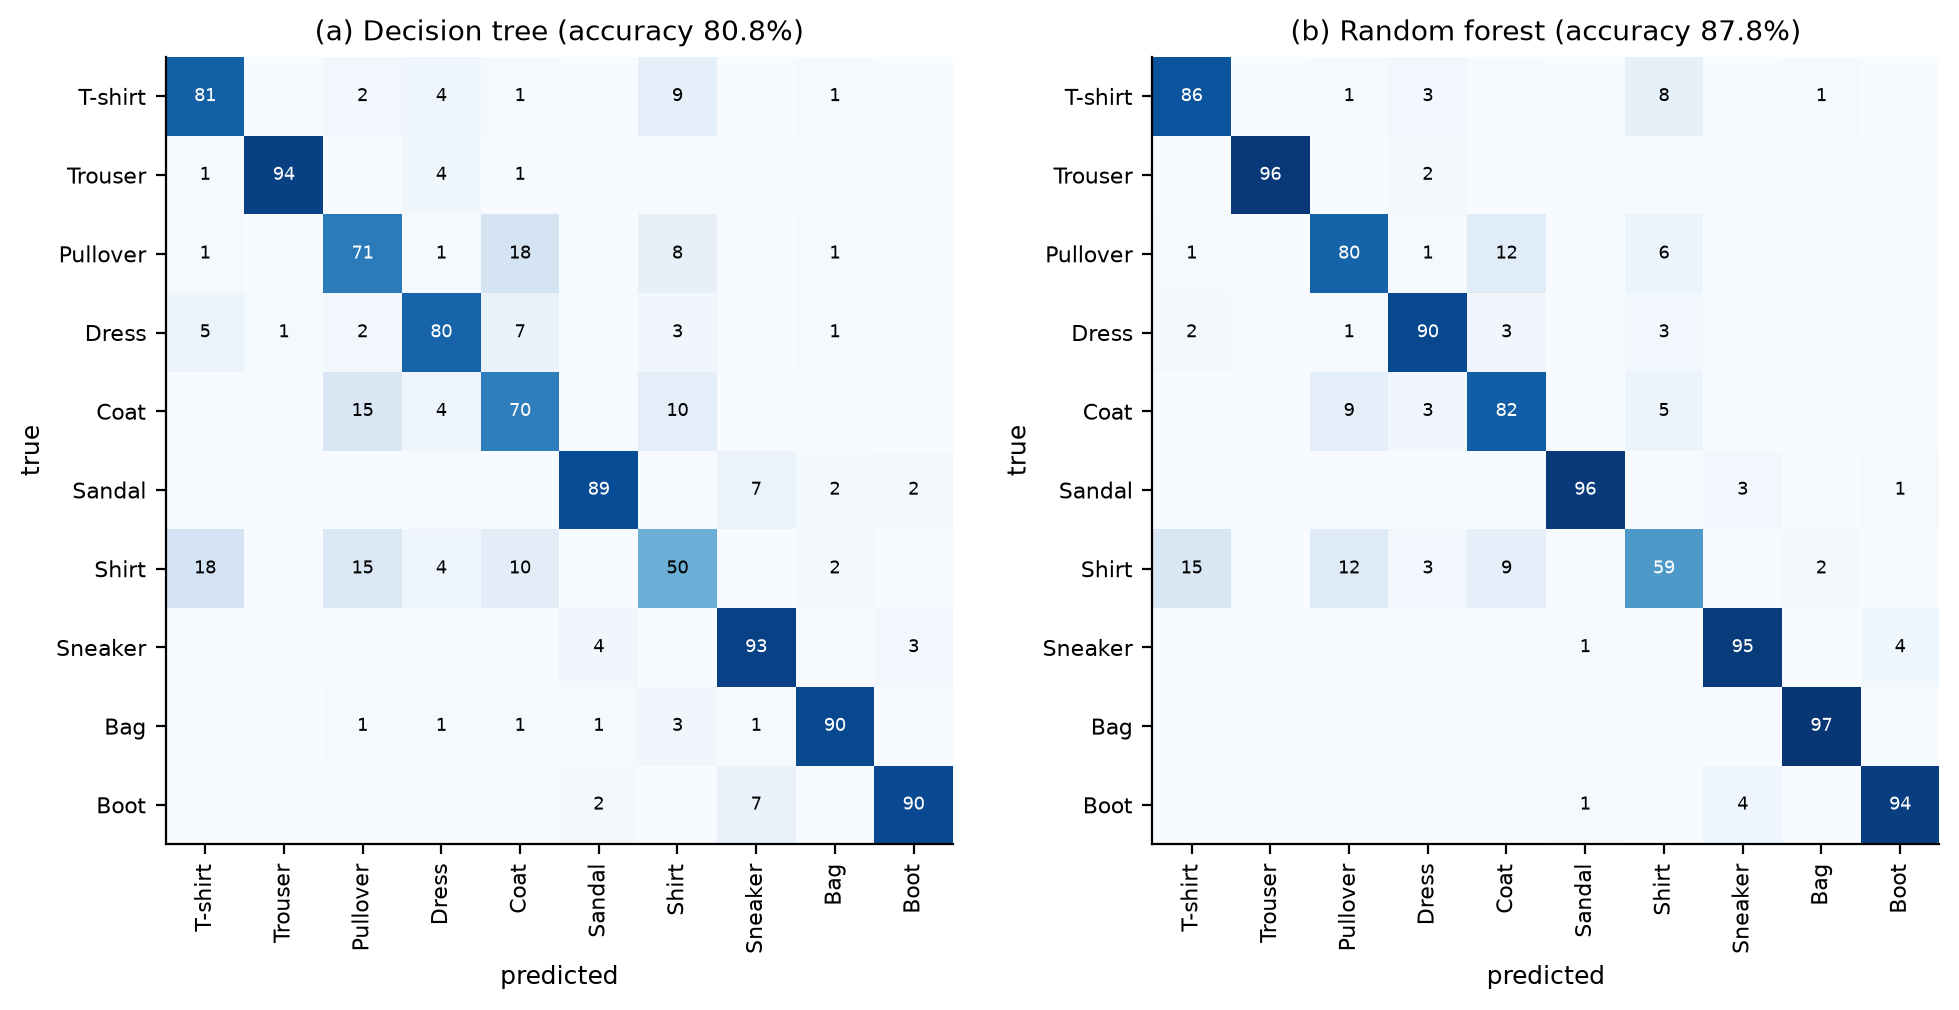
\includegraphics[width=0.92\linewidth]{figures/confusion_matrices.png}
\caption{Row-normalised test confusion matrices (\% of each true class; entries below 1\% left blank).}
\label{fig:cm}
\end{figure}

\begin{figure}[H]
\centering
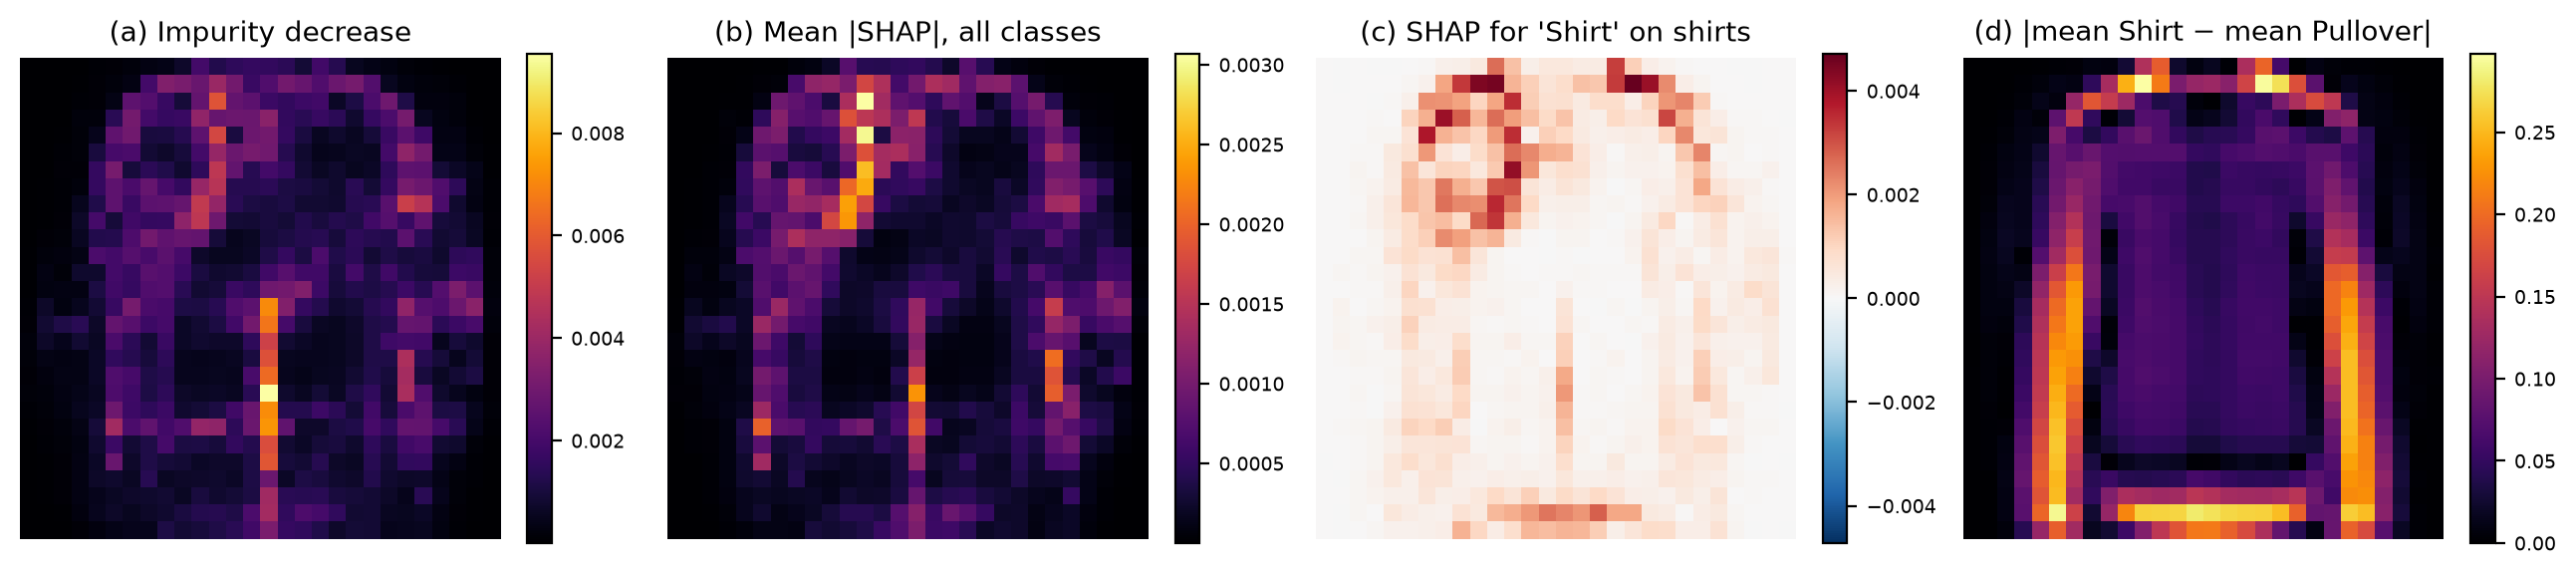
\includegraphics[width=\linewidth]{figures/importance.png}
\caption{(a) Impurity-based importance of the final random forest. (b) Its mean absolute SHAP value over 1{,}000 test images and all classes. (c) Mean SHAP value for the class Shirt on the true shirts among these images (red pushes towards Shirt). (d) Absolute difference between the mean Shirt and mean Pullover images.}
\label{fig:importance}
\end{figure}

\begin{figure}[H]
\centering
\begin{minipage}[t]{0.47\linewidth}
\centering
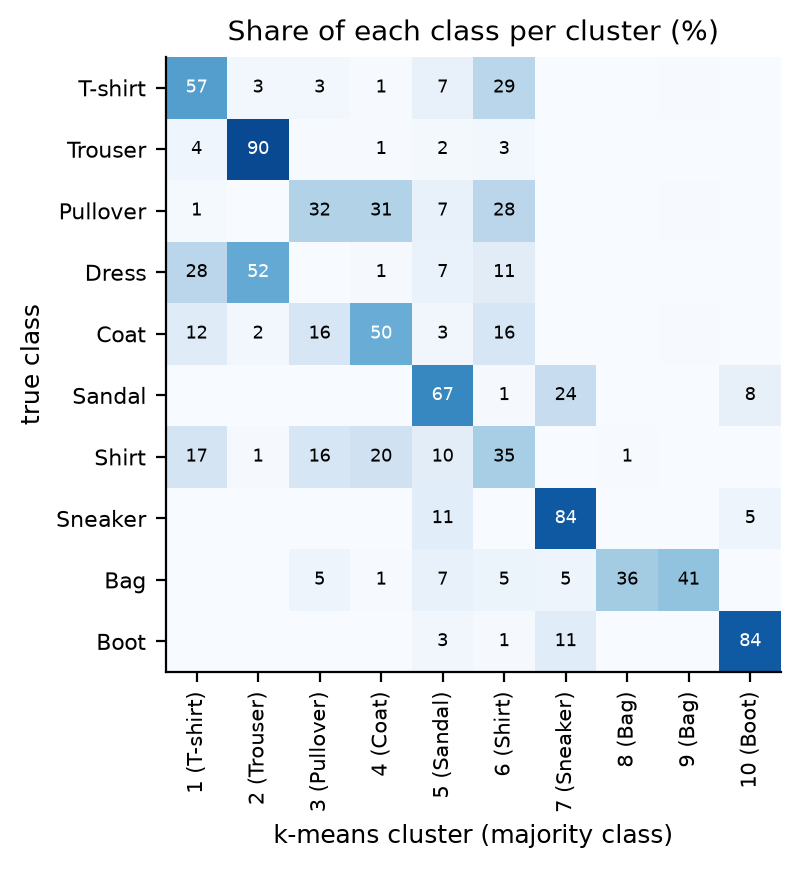
\includegraphics[width=\linewidth]{figures/kmeans.png}
\caption{k-means with ten clusters on the training images: share of every class in each cluster.}
\label{fig:kmeans}
\end{minipage}\hfill
\begin{minipage}[t]{0.5\linewidth}
\centering
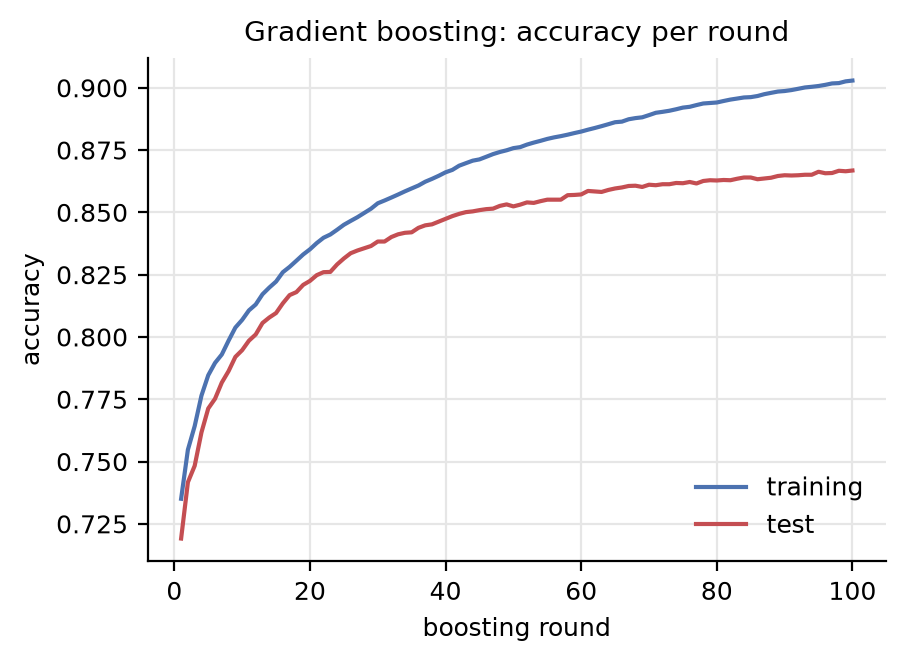
\includegraphics[width=\linewidth]{figures/gb_rounds.png}
\caption{Gradient boosting (default settings, all training data): training and test accuracy after every round.}
\label{fig:gb}
\end{minipage}
\end{figure}

\begin{table}[H]
\centering
\small
\begin{tabular}{lcccccc}
\toprule
Class & Avg.\ image & Tree & Random forest & Grad.\ boosting & XGBoost & CNN check \\
\midrule
T-shirt/top & 0.698 & 0.785 & 0.843 & 0.823 & 0.857 & 0.851 \\
Trouser & 0.924 & 0.956 & 0.980 & 0.977 & 0.983 & 0.985 \\
Pullover & 0.491 & 0.685 & 0.784 & 0.766 & 0.820 & 0.863 \\
Dress & 0.726 & 0.802 & 0.892 & 0.874 & 0.909 & 0.907 \\
Coat & 0.538 & 0.673 & 0.793 & 0.774 & 0.829 & 0.844 \\
Sandal & 0.606 & 0.904 & 0.968 & 0.962 & 0.978 & 0.977 \\
Shirt & 0.263 & 0.541 & 0.649 & 0.642 & 0.709 & 0.738 \\
Sneaker & 0.790 & 0.897 & 0.940 & 0.937 & 0.957 & 0.955 \\
Bag & 0.825 & 0.907 & 0.967 & 0.959 & 0.976 & 0.986 \\
Ankle boot & 0.864 & 0.921 & 0.949 & 0.946 & 0.964 & 0.965 \\
\midrule
Average F1 & 0.672 & 0.807 & 0.877 & 0.866 & 0.898 & 0.907 \\
\bottomrule
\end{tabular}
\caption{Per-class F1 scores on the test set.}
\label{tab:perclass}
\end{table}

\begin{table}[H]
\centering
\small
\begin{tabular}{llr}
\toprule
Layer (Keras) & Output shape & Parameters \\
\midrule
Conv2D(32, $3\times3$, ReLU, padding same), MaxPooling2D($2\times2$) & $14\times14\times32$ & 320 \\
Conv2D(64, $3\times3$, ReLU, padding same), MaxPooling2D($2\times2$) & $7\times7\times64$ & 18{,}496 \\
Flatten, Dense(150, ReLU, L2 penalty), Dropout(0.5) & 150 & 470{,}550 \\
Dense(10, softmax) & 10 & 1{,}510 \\
\midrule
Total & & 490{,}876 \\
\bottomrule
\end{tabular}
\caption{Proposed CNN (augmentation layers in front, active only in training, are not shown).}
\label{tab:cnn}
\end{table}

\subsection*{Check of the CNN design}
\label{app:cnn}
\begin{figure}[H]
\centering
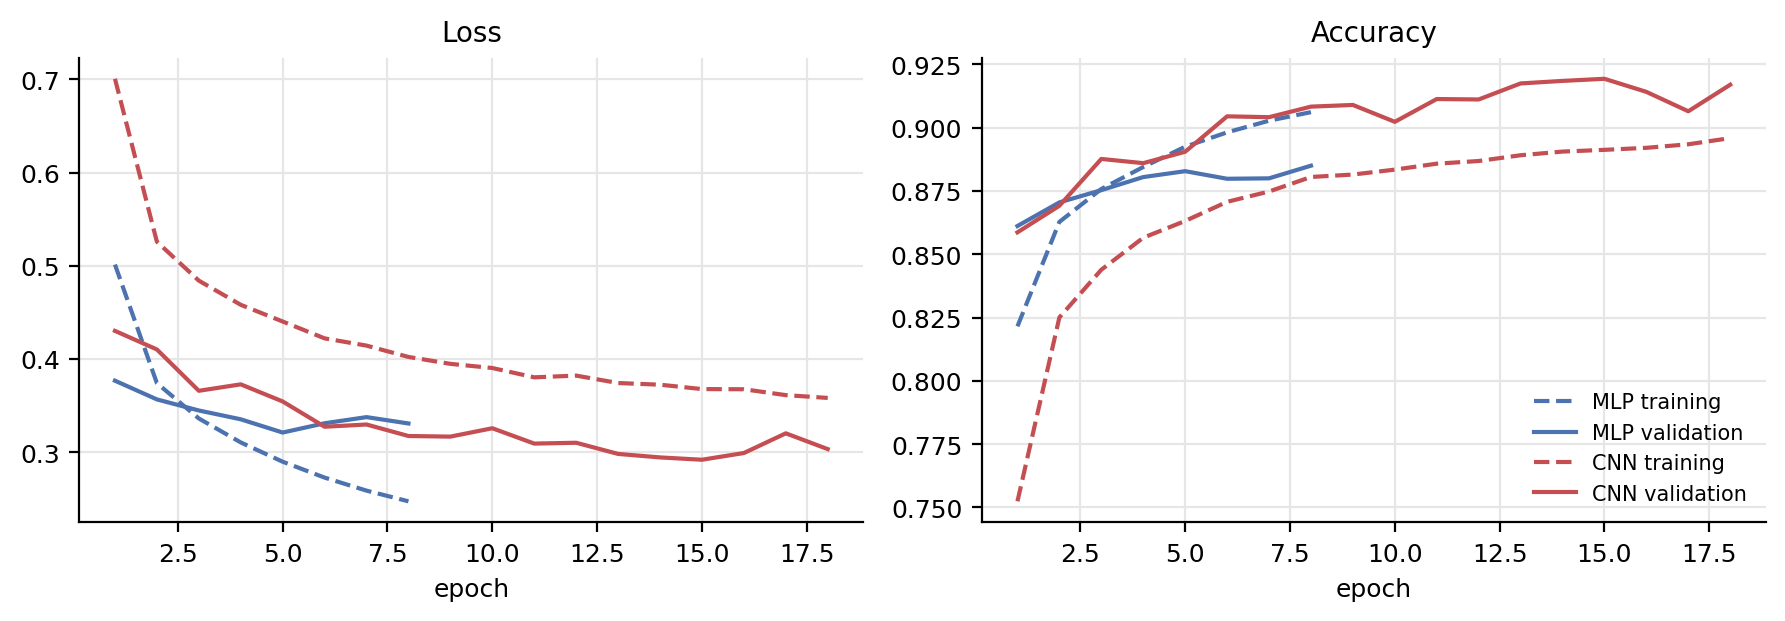
\includegraphics[width=0.85\linewidth]{figures/cnn_history.png}
\caption{Training curves of the proposed CNN and a fully connected network (784--150--60--10), trained once with Adam, batch size 32 and early stopping (patience 3) on a 10\% validation split of the training set. Test accuracy: CNN 90.7\% (18 epochs), fully connected network 86.6\% (8 epochs).}
\label{fig:cnnhist}
\end{figure}


\section{How to run the code}
\label{app:code}
\raggedright
The file \pkg{code.zip} contains two scripts. \pkg{part1\_trees.py} runs all of Part~1: the data analysis, the decision tree, the random forest and bagging, the noise check, the SHAP values, the two boosting references and the training times. It writes all numbers to \pkg{results/part1.json} and produces Figures~\ref{fig:data}--\ref{fig:gb}. \pkg{part2\_cnn\_check.py} trains the proposed CNN and the fully connected network once (Figure~\ref{fig:cnnhist}). The data are loaded with \pkg{keras.datasets.fashion\_mnist.load\_data()}, which downloads Fashion-MNIST on the first run. To reproduce the results:
\begin{enumerate}[leftmargin=*,itemsep=1pt,topsep=2pt]
\item Install Python 3.11 or newer and the packages \pkg{numpy} (2.4.4), \pkg{scikit-learn} (1.8.0), \pkg{matplotlib} (3.10.9), \pkg{shap} (0.52.0), \pkg{xgboost} (3.4.1) and \pkg{tensorflow} (2.21.0), for example with \pkg{pip install}.
\item From inside \pkg{code/}, run \pkg{python part1\_trees.py} (about 3 hours on a laptop, most of it for gradient boosting) and \pkg{python part2\_cnn\_check.py} (about one hour).
\end{enumerate}
All random seeds are fixed (\pkg{random\_state=42}), so the numbers in this report are reproduced with these package versions.

\end{document}
